\documentclass[11pt]{article}
\usepackage[T1]{fontenc}
\usepackage{amsmath,amssymb}
\usepackage[margin=1in]{geometry}
\usepackage{graphicx}
\usepackage{float}
\usepackage[hidelinks]{hyperref}
\setlength{\parindent}{0pt}
\setlength{\parskip}{6pt}
\newcommand{\run}[1]{\texttt{\detokenize{#1}}}
\title{\textbf{Vanilla vs LUT47:\\ what changes inside the model when the MLP FFN becomes a LUT}}
\author{ffn\_replacement interpretability analysis}
\date{\today}

\begin{document}
\maketitle

\textbf{Models} (both \texttt{MinimalGPT}, $E{=}384$, attention $H{=}6$, depth 6, RoPE, ClimbMix, same tokenizer):
\begin{itemize}
\item \textbf{A) Vanilla} --- standard dense-MLP FFN. Run \run{exp_n_0216_vanilla48k_gelu_ckpt2k_seed1}, val\_bpb \textbf{1.1151}.
(The task named \run{exp_n_0177_vanilla48k_corrected}, but that folder has \emph{no} checkpoint; 0216 is the substitute --- a 48K vanilla with an essentially identical val\_bpb 1.115094 vs 1.115092 --- and it has weights saved.)
\item \textbf{B) LUT47} --- FFN replaced by a light CompressionMultiHeadLUT (H8/tph64, nap8, read\_top\_n=2, float read, dropout+TV). Run \run{exp_n_abl_47_B48k_light_lmfrozeng_n2_tau0p5_tv10_tph64_h8_seed1_noquant_headdrop20}, val\_bpb \textbf{1.1079} (beats vanilla by 0.0072).
\end{itemize}

Both checkpoints load with missing=0/unexpected=0 and run forward passes; all activations captured via forward hooks on the identical attention path and on the FFN slot. Shared eval batch: $8\times256$ real ClimbMix val tokens, same tokens to both models.

\section{Attention patterns}
The attention \emph{architecture} is identical, so any systematic difference is \textbf{demanded by the FFN}.
The LUT model's attention is systematically \textbf{sharper} (lower entropy): mean 3.10 bits (LUT) vs 3.60 (vanilla), sharpest at layers 1/2/5. Layer 0 is diffuse in both ($\sim$5.7 bits). Induction heads exist in both at comparable strength ($\sim$0.14), slightly relocated (vanilla L3H1, LUT L4H0); max previous-token attention 0.575 vs 0.487.
\emph{Takeaway:} a discrete/low-rank LUT read wants cleaner, more decisive inputs, so the shared attention learns to be sharper.

\begin{figure}[H]\centering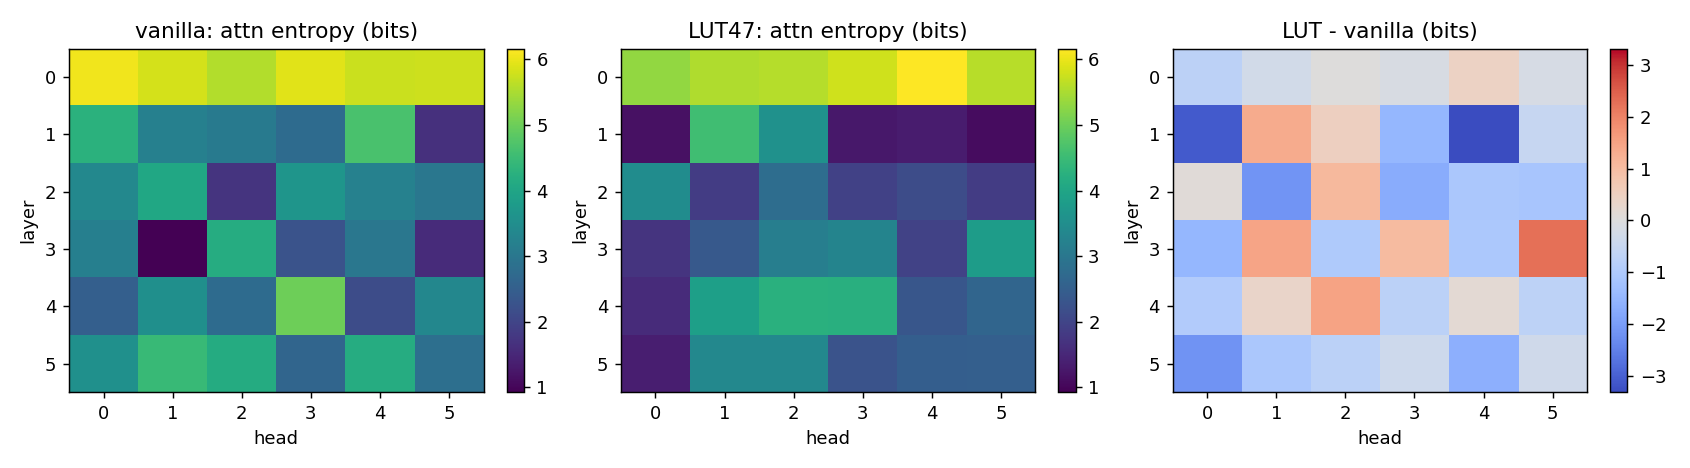
\includegraphics[width=\linewidth]{attn_entropy_heatmaps.png}
\caption{Per-(layer, head) mean attention entropy (bits): vanilla, LUT, and their difference. Blue in the diff = the LUT sharpens that head.}\end{figure}

\begin{figure}[H]\centering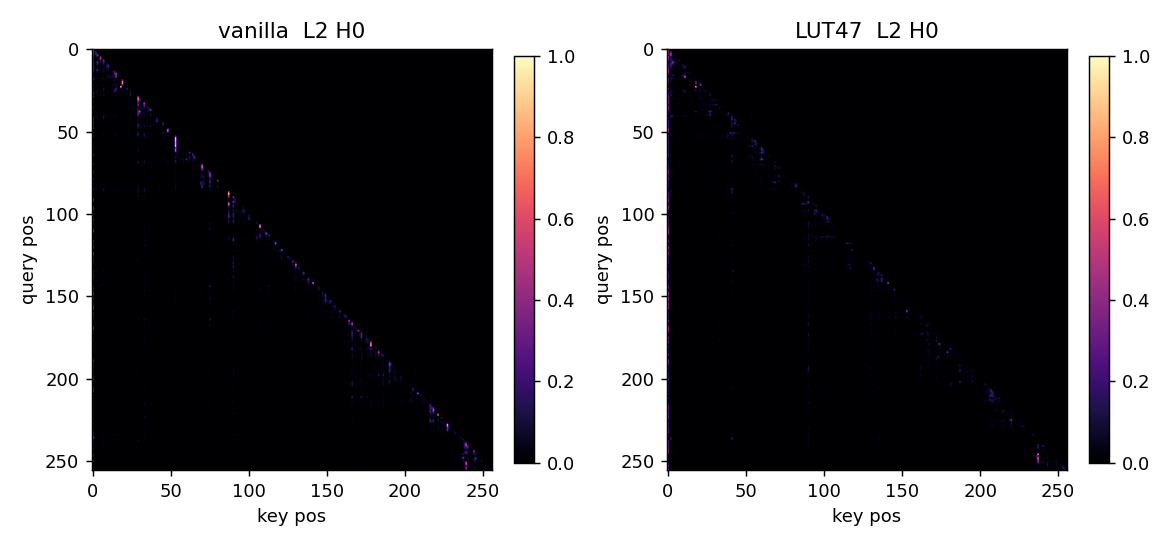
\includegraphics[width=0.85\linewidth]{attn_examples.png}
\caption{Example attention heatmap (layer 2, head 0) on the shared batch.}\end{figure}

\section{Embeddings}
Separately trained, so absolute directions do not align --- comparing \emph{structure}.
Token embeddings are near-full-rank and near-isotropic in both (effective rank $\approx$342 (vanilla) vs 333 (LUT) out of 384; isotropy 0.14 vs 0.17). The untied unembedder is \textbf{low-rank and highly anisotropic in both, and nearly identical} (effective rank $\approx$63, isotropy $\approx$0.89 --- the usual dominant ``rogue direction''). \emph{Takeaway:} swapping the FFN barely touches the embedding/unembedding geometry.

\begin{figure}[H]\centering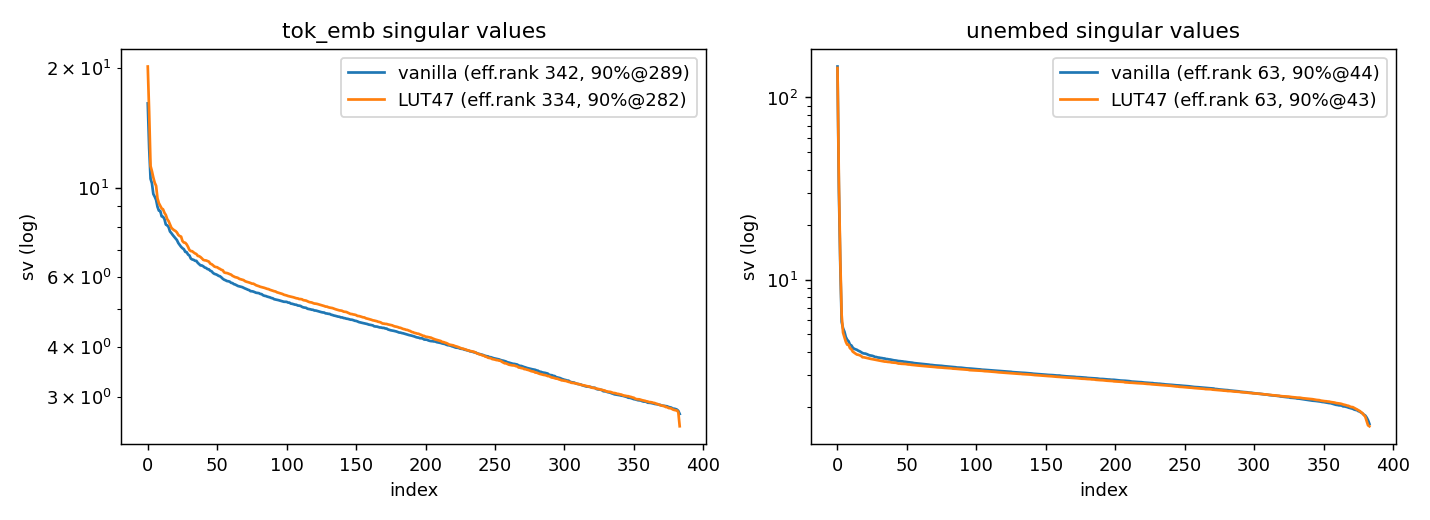
\includegraphics[width=\linewidth]{embed_svspectrum.png}
\caption{Singular-value spectra (log) of the token embedding and the untied unembedder, with effective rank. The unembedder is far lower-rank than the token embedding and is essentially the same for both models.}\end{figure}

\begin{figure}[H]\centering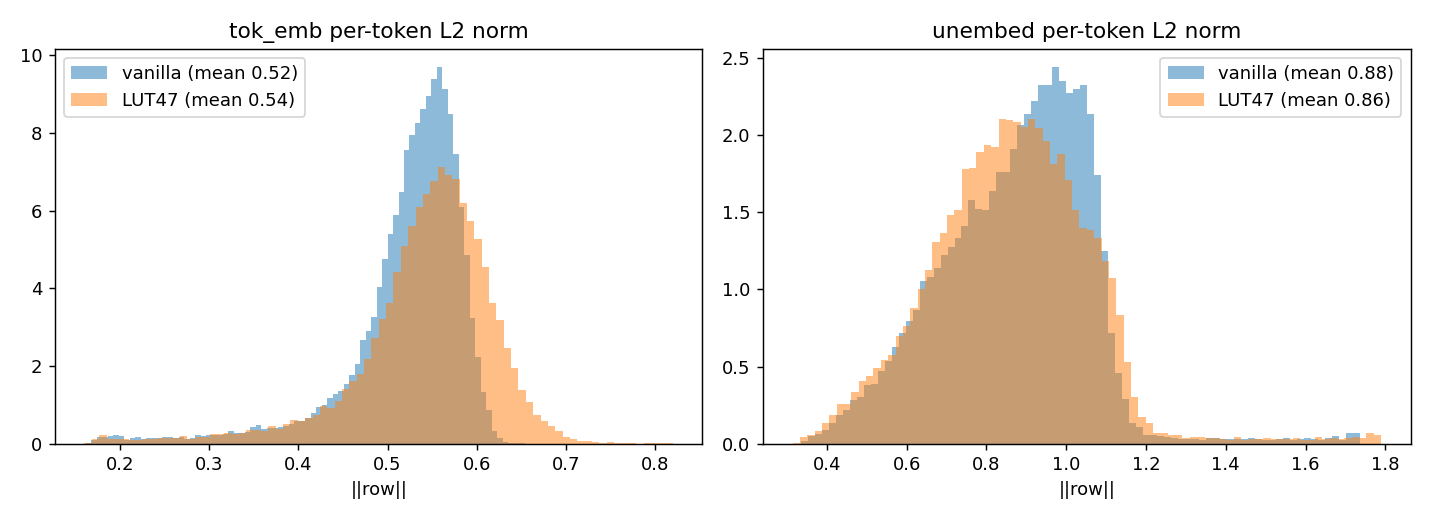
\includegraphics[width=\linewidth]{embed_norms.png}
\caption{Per-token L2-norm distributions for the token embedding and unembedder.}\end{figure}

\section{FFN vs LUT internals --- the biggest differences}
The LUT FFN writes \textbf{much smaller residual updates} and the model runs at a \textbf{smaller residual scale}: mean $\lVert\text{FFN }\Delta\rVert$ per layer vanilla $[5.5,3.3,3.6,4.5,5.9,12.8]$ vs LUT $[0.6,1.6,1.1,1.3,1.9,5.4]$; residual norm up to 18.2 (vanilla) vs 9.9 (LUT); ratio $\Delta$/residual $\approx$0.4--0.95 (vanilla) vs 0.2--0.55 (LUT). The LUT updates are also \textbf{low-rank, especially early}: effective rank $[5.5,7.4,188,194,184,24]$ (LUT) vs $[225,111,261,259,249,139]$ (vanilla) --- the early LUT layers write into a $\sim$5--7 dimensional subspace, the signature of a discrete lookup. The LUT read is sparser than the dense GELU hidden, most at layer 0 (16.6\% near-zero vs $<$1\%).
\emph{Takeaway:} the LUT is a lighter, lower-rank, sparser operator than the MLP; it moves the residual less and in fewer directions.

\begin{figure}[H]\centering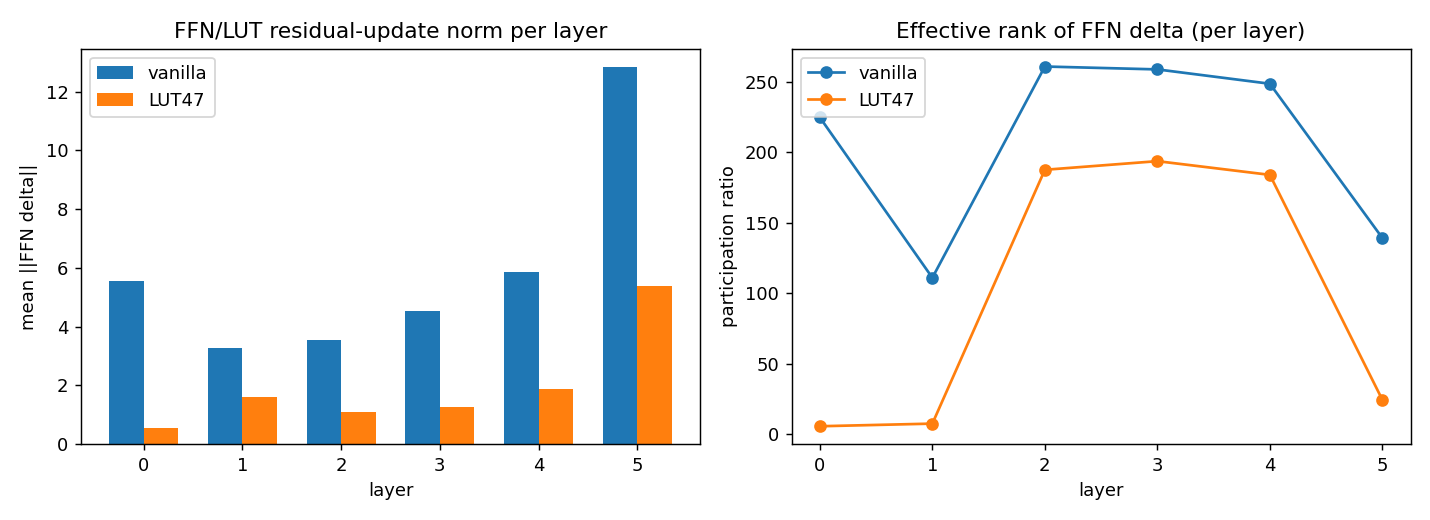
\includegraphics[width=\linewidth]{ffn_delta.png}
\caption{Left: per-layer FFN residual-update norm (the LUT writes far less than the MLP). Right: effective rank of the FFN update --- the LUT's early layers are strikingly low-rank.}\end{figure}

\begin{figure}[H]\centering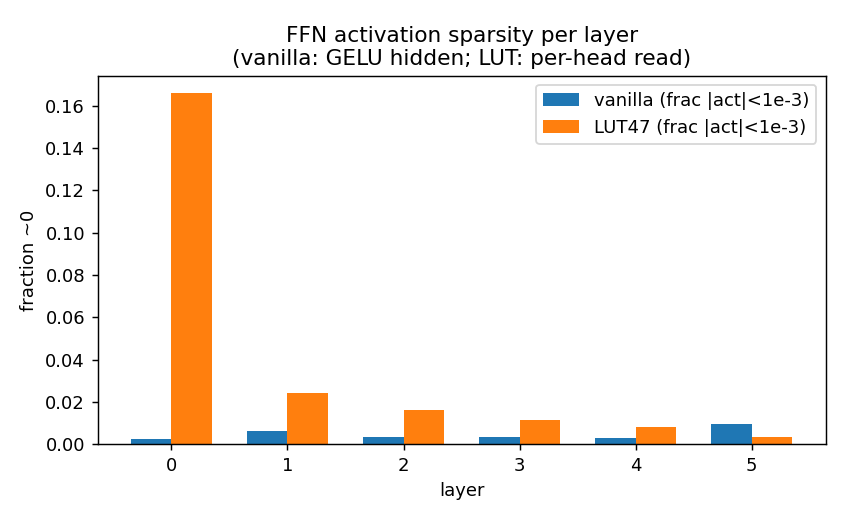
\includegraphics[width=0.7\linewidth]{ffn_sparsity.png}
\caption{Per-layer FFN activation sparsity (fraction near zero): the LUT read is sparser early.}\end{figure}

\section{Single-sentence trace}
Side-by-side on \texttt{The capital of France is} and \texttt{The cat sat on the mat.}: next-token top-5, per-layer attn/FFN/residual norms, and per-head attention (full detail in \texttt{sentence\_trace.md}). It confirms the aggregate picture: on the France prompt the LUT FFN's final-layer update is 2.38 vs the vanilla 10.38 ($\Delta$/residual 0.19 vs 0.53), and the LUT's layer-5 heads attend $\sim$0.90 to the last token while the vanilla heads spread across `is'/`of'/`capital'. Neither small ClimbMix model actually predicts ``Paris'' --- both are weak; this is about mechanism, not factual recall.

\begin{figure}[H]\centering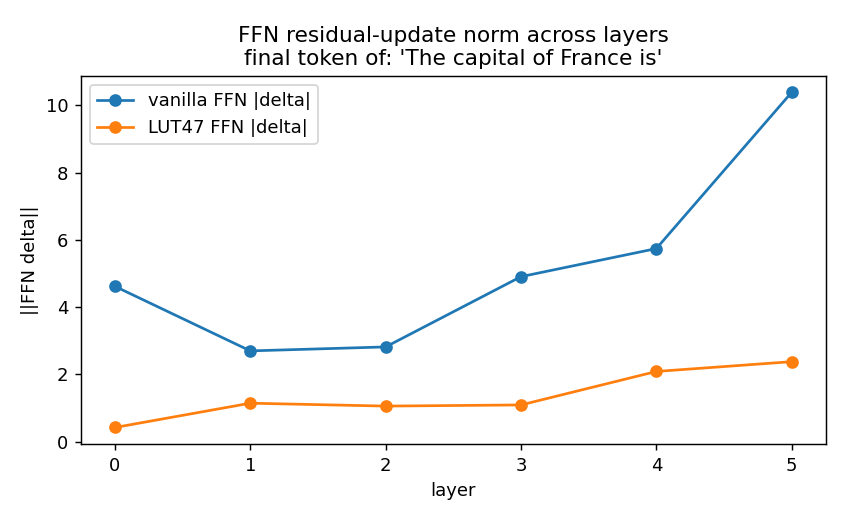
\includegraphics[width=0.7\linewidth]{trace_ffn_delta.png}
\caption{FFN residual-update norm across layers on the final token of ``The capital of France is''.}\end{figure}

\section{Per-head LightMHL FFN characterization (LUT47, H8/tph64)}
Each LightMHL head of the FFN LUT is a map $\mathbb{R}^{48}\!\to\!\mathbb{R}^{48}$ (its 48-dim input code slice
$\to$ its 48-dim top-$n$-blended read, \emph{before} decompress). Confirmed dims: 6 layers $\times$ 8 heads,
tph=64 tables/head, nap=8 ($2^8{=}256$ cells/table), input\_dim/head = output\_dim/head = 48. Driven on
$16\times256$ real ClimbMix tokens; cell selections captured by disabling the compiled path and wrapping
\texttt{\_pack\_index}.

\textbf{Findings.}
\begin{itemize}
\item \textbf{Codebook usage is DENSE, not sparse.} Across the batch $\sim$16{,}000 of the 16{,}384 possible
(table, cell) selections fire ($\sim$97\%), with cell-selection entropy $\sim$13.4 of a max 14 bits. It is
\emph{not} ``a few cells fire'': nearly the whole codebook is exercised; the moderate output rank comes from
cell \emph{values} clustering, not from sparse addressing.
\item \textbf{Per-head output rank is $\cap$-shaped with depth}: mean effective rank 27 (L0) $\to$ 46--47 (L2--4,
near-full 48) $\to$ 38 (L5). Note this is \emph{per head before decompress}; the full residual write collapses much
lower ($\sim$5--7 early, \S3) because the learned dense decompress projects the correlated head outputs into a
low-dim subspace at early layers --- a learned collapse, not a structural cap (H8 has $8{\times}48{=}384$, no bottleneck).
\item \textbf{Not single-table piecewise-constant.} A single table's selected cell explains only 11--29\% of the
head-output variance (each head sums 64 tables plus a top-2 blend), so the read is a dense sum of many discrete
selections rather than one switch.
\item \textbf{Magnitude grows with depth}, sparsity falls: per-head $\lVert$output$\rVert$ 0.08 $\to$ 2.3 from L0 to
L5; near-zero read fraction 16.6\% (L0) $\to$ 0.3\% (L5).
\item \textbf{Heterogeneity at the ends.} Early (L0) and late (L5) layers contain some \emph{near-dead} heads
(output rank $\sim$2--4, tiny norm) alongside rich ones (rank $\sim$38--45); the middle layers (L2--4) are uniformly
rich (rank $\sim$46 for all 8 heads). Specialization/dead heads concentrate at the ends; the middle is a uniform,
high-rank workhorse.
\end{itemize}

\begin{figure}[H]\centering
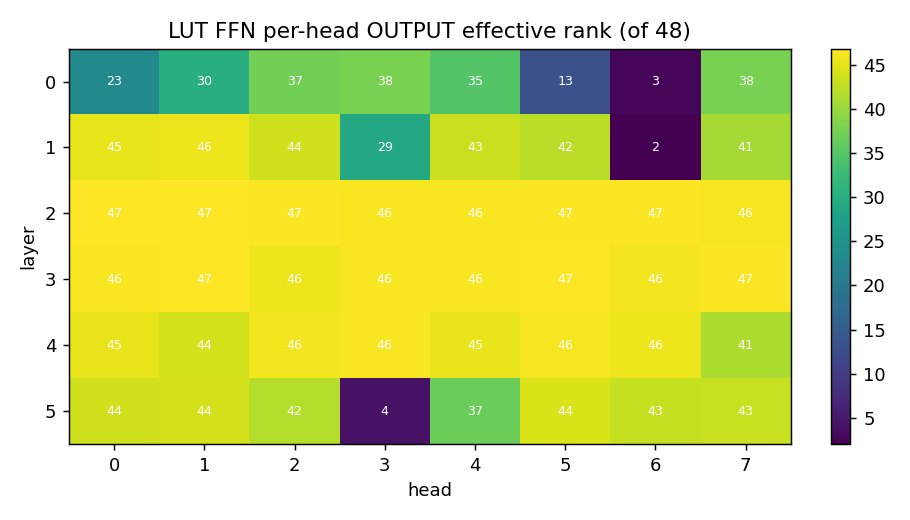
\includegraphics[width=0.49\linewidth]{ph_output_rank.png}\hfill
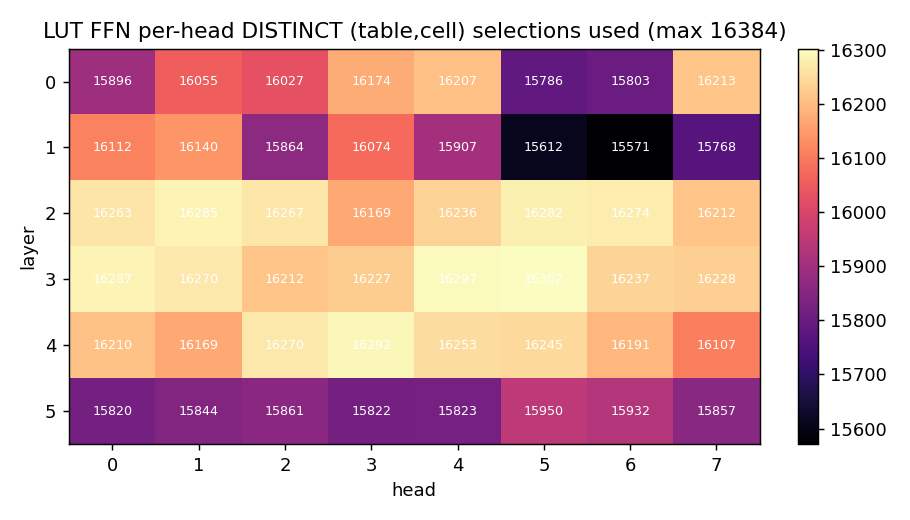
\includegraphics[width=0.49\linewidth]{ph_distinct_cells.png}
\caption{Per-(layer,head): output effective rank (left; note the near-dead heads at L0/L5 and the uniform middle) and
distinct (table,cell) selections used (right; near-saturated $\sim$16k/16{,}384 everywhere = dense codebook usage).}\end{figure}

\begin{figure}[H]\centering
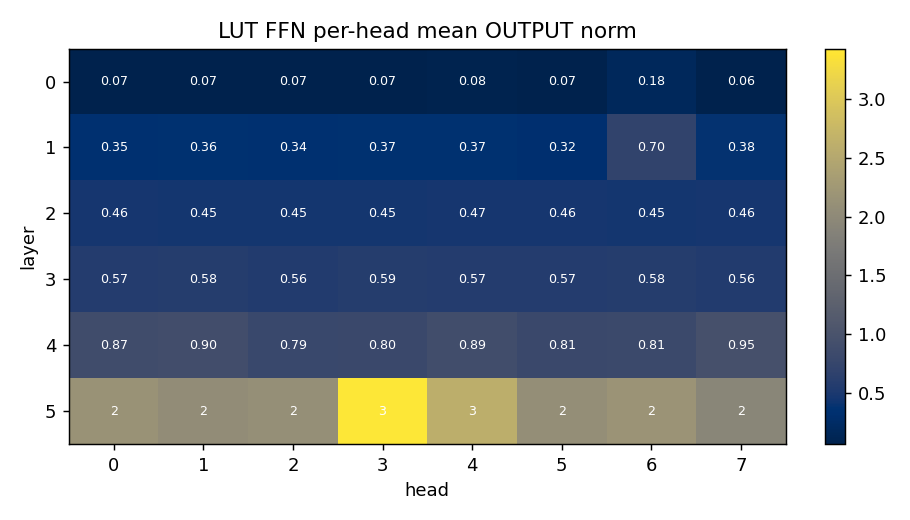
\includegraphics[width=0.49\linewidth]{ph_output_norm.png}\hfill
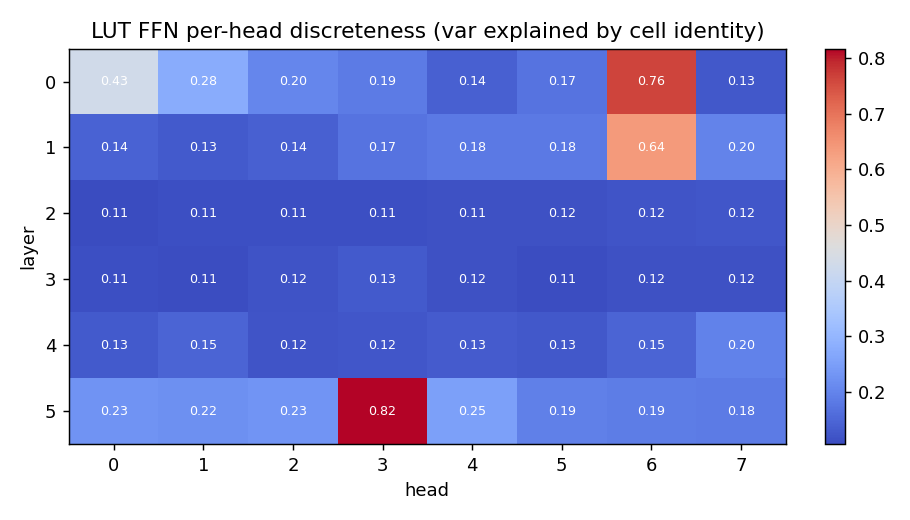
\includegraphics[width=0.49\linewidth]{ph_discreteness.png}
\caption{Per-(layer,head): mean output norm (left; grows with depth) and discreteness --- fraction of output variance
explained by one table's cell identity (right; low, i.e. the read is a dense sum of many selections).}\end{figure}

\begin{figure}[H]\centering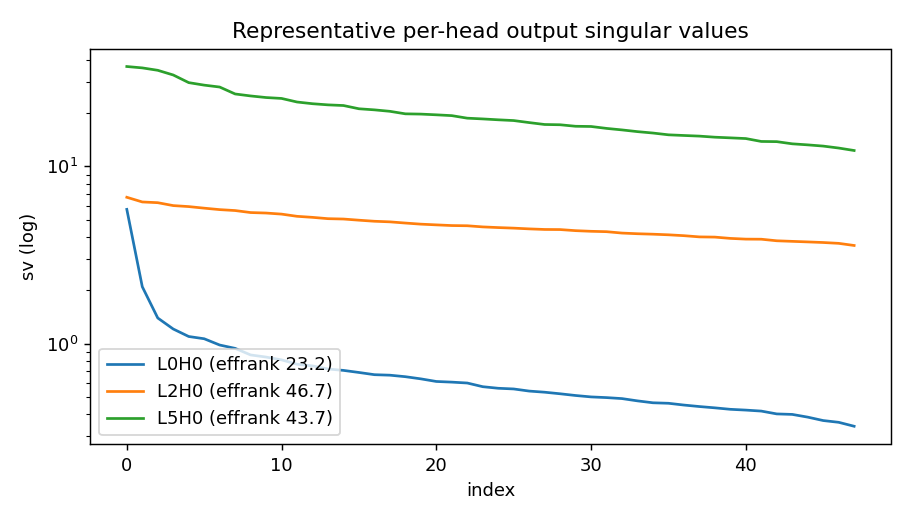
\includegraphics[width=0.7\linewidth]{ph_svspectra.png}
\caption{Representative per-head output singular-value spectra (L0/L2/L5, head 0).}\end{figure}

\subsection{Why the early residual write collapses to rank $\sim$5--7}
The FFN residual write is $\text{write}=W_{\text{dec}}\cdot(\text{concat of the 8 head reads})$. For this H8 model the
concatenated code is $8\times48=384$-dim and $W_{\text{dec}}$ is a full dense $384\times384$ (no structural bottleneck).
We decomposed the write rank per layer into: rank of the joint 384-d code, (stable) rank of $W_{\text{dec}}$, rank of the
write, and cross-head read correlation.

\begin{center}\small
\begin{tabular}{c|cc|cc|ccc|c}
L & code eff.rank & code r99 & write eff.rank & write r99 & $W_{\text{dec}}$ eff.rank & $W_{\text{dec}}$ stable & $W_{\text{dec}}$ r99 & mean off-diag $|\!\cos\!|$ \\ \hline
0 & 19.4 & 98  & 5.6   & 5   & 218 & 20.9 & 259 & 0.115 \\
1 & 21.6 & 148 & 7.3   & 13  & 245 & 35.6 & 276 & 0.117 \\
2 & 344.7& 371 & 193.8 & 246 & 242 & 54.7 & 274 & 0.116 \\
3 & 344.4& 372 & 199.9 & 248 & 243 & 68.6 & 274 & 0.116 \\
4 & 323.1& 370 & 188.0 & 243 & 251 & 70.3 & 278 & 0.116 \\
5 & 61.0 & 274 & 25.6  & 102 & 259 & 45.7 & 285 & 0.116 \\
\end{tabular}
\end{center}

\textbf{Mechanism.} The collapse is driven mainly by the \textbf{joint code}, not by $W_{\text{dec}}$: at L0--L1 the concatenated
384-d head-read code has effective rank only $\sim$19--22 (99\% energy in $\sim$98--148 dims), even though each head's 48-d read
is individually rank $\sim$27--46. The 8 heads are \emph{not} strongly pairwise-correlated (mean off-diagonal read $|\!\cos\!|\approx0.12$
at every layer) --- the redundancy is a \emph{shared low-dimensional structure} across heads, not pairwise duplication. $W_{\text{dec}}$
is near-full-rank at every layer (r99 $\sim$274--285), so it is \textbf{not} a structural bottleneck; but it is anisotropic, and early
its \emph{stable} rank is low ($\sim$21), which \emph{compounds} the collapse --- it concentrates the already-low-rank code down from
$\sim$20 to the $\sim$5--6-dim write. Middle layers (L2--4) do not collapse because the joint code becomes near-full-rank ($\sim$323--345)
and $W_{\text{dec}}$'s stable rank rises ($\sim$55--70). \textbf{Why early vs middle:} early layers haven't yet built a rich residual, so
the LUT reads have little to differentiate on --- the joint code lives in a $\sim$20-d subspace and the FFN barely moves the residual
(\S3); by the middle the residual carries rich information, the reads span the full space, and the write is rich. L5 partially
re-collapses (code 61, write 26) as the network narrows toward the output.

\begin{figure}[H]\centering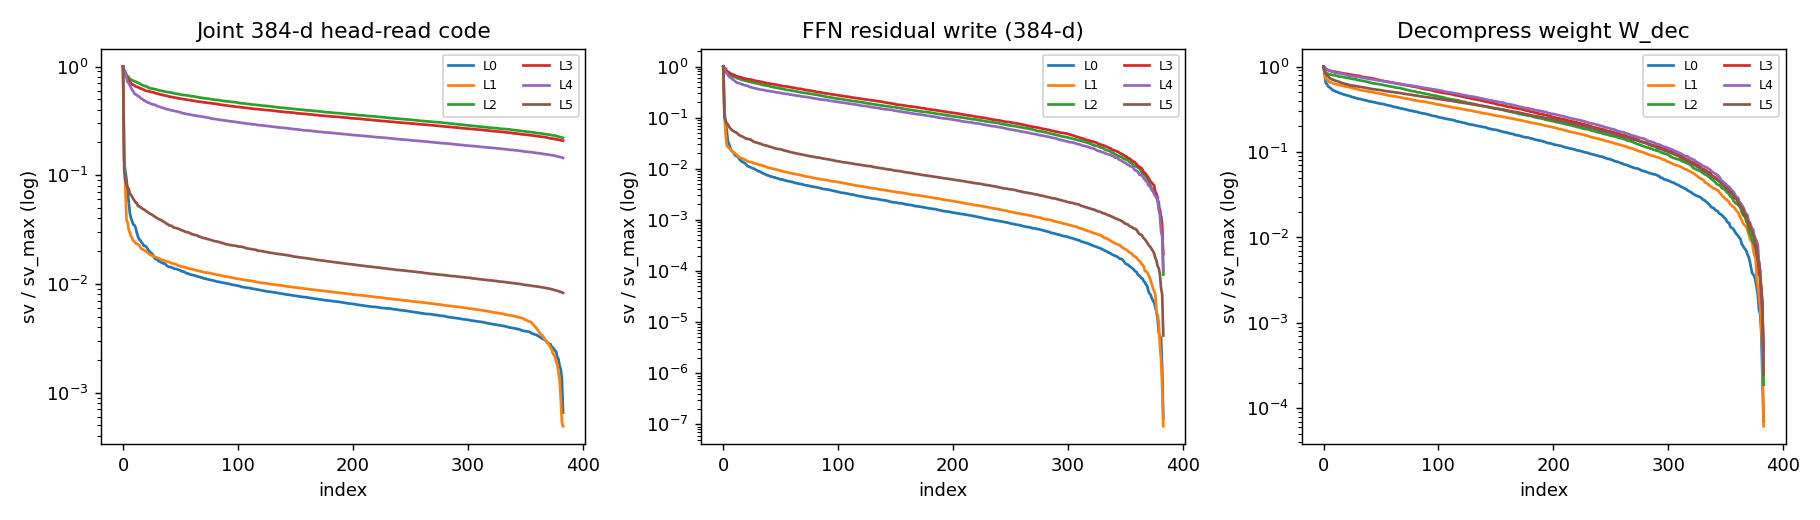
\includegraphics[width=\linewidth]{collapse_svd.png}
\caption{Per-layer normalized singular-value spectra: joint 384-d head-read code (left), the 384-d FFN write (middle), and the
decompress weight $W_{\text{dec}}$ (right). The code and write spectra drop off a cliff at L0/L1 (low rank) and are full at L2--4;
$W_{\text{dec}}$ is near-full-rank at all layers.}\end{figure}

\begin{figure}[H]\centering
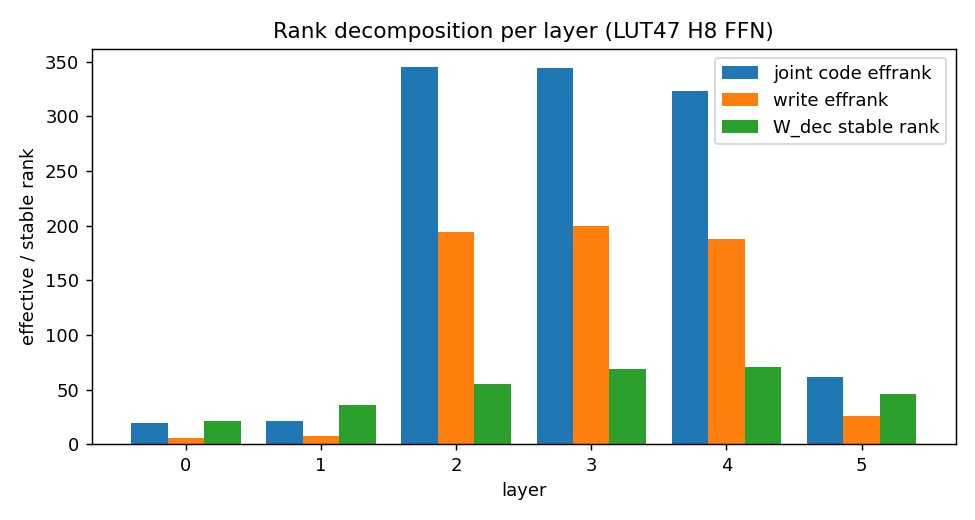
\includegraphics[width=0.52\linewidth]{collapse_ranks.png}\hfill
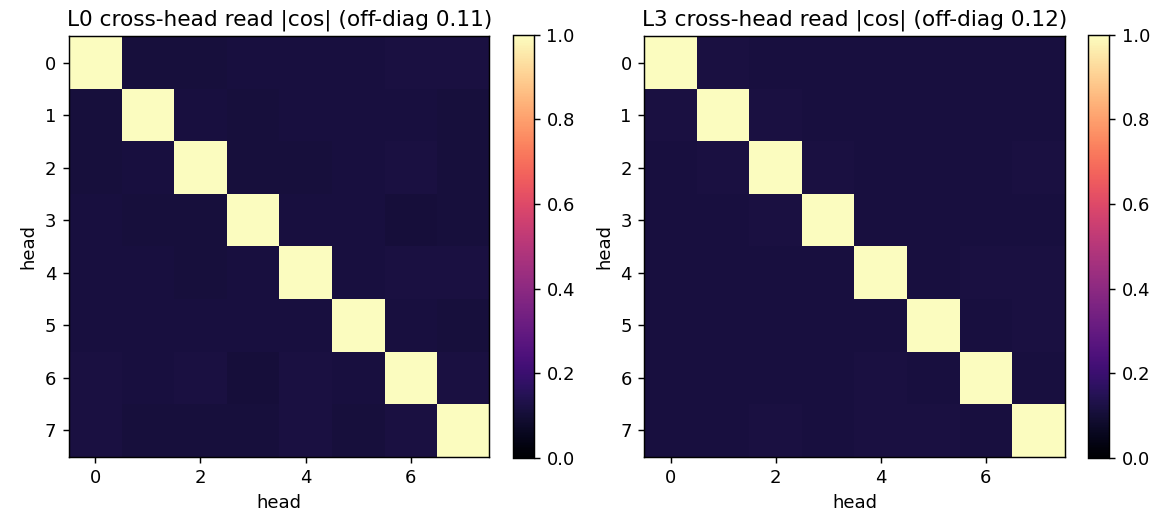
\includegraphics[width=0.46\linewidth]{collapse_crosshead.png}
\caption{Left: joint-code effective rank, write effective rank, and $W_{\text{dec}}$ stable rank per layer --- the write tracks the
JOINT CODE, not $W_{\text{dec}}$. Right: cross-head read $|\!\cos\!|$ heatmaps at the collapsed L0 vs the rich L3 --- both low and
similar ($\sim$0.12 off-diagonal), i.e. the collapse is not pairwise head correlation.}\end{figure}

\subsection{Per-table structure: is the early low rank baked into the tables?}
Each head has 64 tables; each table stores $2^{8}{=}256$ cells of $d_{\text{out}}{=}48$ value vectors (constant cells).
We compare the STATIC structure (what the stored values can span) with the DATA-DRIVEN structure (what actually fires),
per layer:

\begin{center}\small
\begin{tabular}{c|c|c|c|c}
L & per-table rank ($\pm$sd, of 48) & within-head cross-table overlap & STATIC union rank & DATA output rank \\ \hline
0 & 42.0 $\pm$0.5 & 0.34 & 45.6 & 27.1 \\
1 & 42.1 $\pm$0.5 & 0.30 & 46.4 & 36.5 \\
2 & 44.6 $\pm$0.3 & 0.26 & 47.7 & 46.6 \\
3 & 44.6 $\pm$0.3 & 0.25 & 47.7 & 46.4 \\
4 & 44.3 $\pm$0.3 & 0.25 & 47.7 & 45.1 \\
5 & 43.9 $\pm$0.3 & 0.24 & 47.7 & 37.6 \\
\end{tabular}
\end{center}

\textbf{Answer: the early low rank is DATA-DRIVEN, not baked into the tables.}
\begin{itemize}
\item Each table is INDIVIDUALLY HIGH-RANK --- effective rank $\sim$42--45 of 48 at every layer. Not low-rank tables.
\item Tables within a head share only MODERATE subspace overlap (0.34 early $\to$ 0.24 late, where 0 = orthogonal, 1 =
identical). They do \emph{not} collapse onto the same few directions.
\item STATICALLY, the 64 tables jointly span $\sim$46--48 of the 48 dims at EVERY layer (union rank), including L0 --- the
codebooks are rich everywhere.
\item Yet the DATA-DRIVEN per-head output is only 27 at L0 vs a static span of 46. The gap is the whole story: the early-layer
inputs select cells whose \emph{realized} (top-2-blended, small-magnitude) reads span a lower-dim subspace, even though the tables
\emph{could} produce $\sim$46. By L2--4 the data exercises the full static span (46.6 $\approx$ 47.7). So the $\cap$-shaped output
rank is a property of WHICH cells fire on real tokens, consistent with the collapse analysis (early residual is thin, so the reads
have little to differentiate) --- it is \emph{not} that each table is low-rank or that all tables share a few directions.
\end{itemize}

\begin{figure}[H]\centering
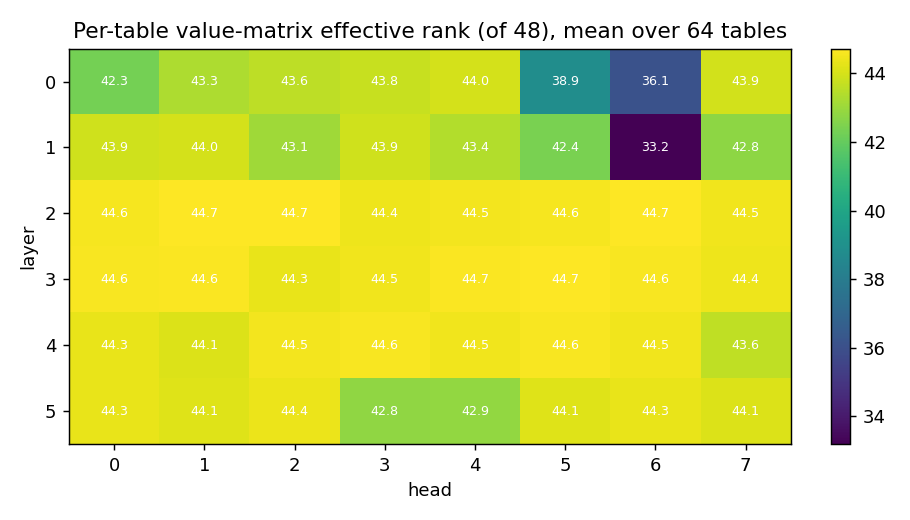
\includegraphics[width=0.49\linewidth]{pt_pertable_rank.png}\hfill
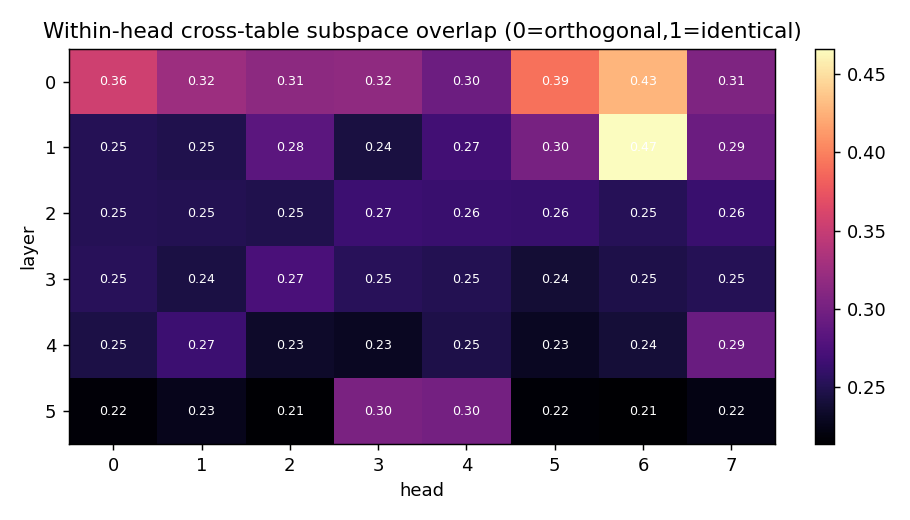
\includegraphics[width=0.49\linewidth]{pt_overlap.png}
\caption{Per-(layer,head): mean per-table value-matrix rank (left; high, $\sim$42--45 everywhere) and within-head cross-table
subspace overlap (right; moderate, $\sim$0.24--0.34 --- tables are not redundant).}\end{figure}

\begin{figure}[H]\centering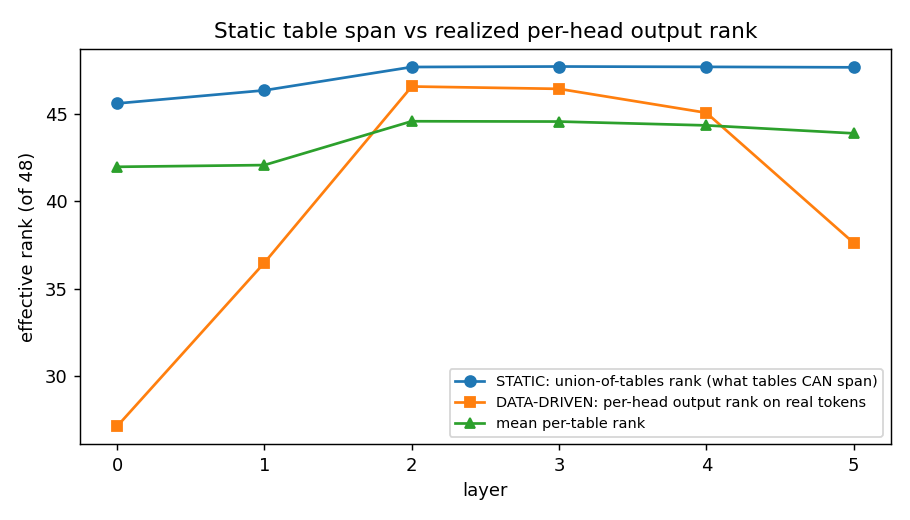
\includegraphics[width=0.72\linewidth]{pt_static_vs_data.png}
\caption{Static union-of-tables span ($\sim$46--48 at all layers) vs the realized per-head output rank on real tokens
($\cap$-shaped 27$\to$46$\to$38). The large L0/L1/L5 gap = the low rank is data-driven, not a table property.}\end{figure}

\section{Overall}
Replacing the MLP with a LUT FFN \textbf{shifts work out of the FFN} (smaller, lower-rank, sparser residual writes) and \textbf{demands sharper attention}, while leaving the token/unembedding geometry essentially unchanged --- and it slightly \textbf{wins} on val\_bpb (1.1079 vs 1.1151). The LUT behaves like a decisive, low-rank router that offloads mixing onto a crisper attention path.

\end{document}
